\documentclass{standalone}
\usepackage{tikz}
\begin{document}
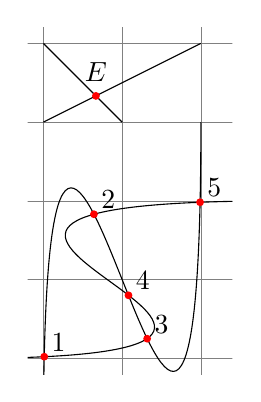
\begin{tikzpicture}[
    every node/.style={fill=red,circle,inner sep=1pt,}]
\clip (.8,.8) rectangle (3.4,5.2);
\draw[help lines] (0,0) grid (4,6);

\usetikzlibrary{intersections}

\draw[name path=P] (1,4) -- +(2,1);
\draw[name path=Q] (2,4) -- +(-1,1);
\path[name intersections={of=P and Q,by=W}];
\node[label=90:$E$] at (W) {};

\draw[name path=A] (0,1)..controls ++(6.5,0) and ++(-7,0)..(4,3);
\draw[name path=B] (1,0)..controls ++(0,9) and ++(0,-9)..(3,4);
\fill[name intersections={of=A and B, name=C, total=\t}]
    \foreach \s in {1,...,\t}{
        (C-\s) node[label=45:\s] {}
    };

\end{tikzpicture}
\end{document}
